\documentclass[10pt,twocolumn,letterpaper]{article}

\usepackage{cvpr}
\usepackage{times}
\usepackage{epsfig}
\usepackage{graphicx}
\usepackage{amsmath}
\usepackage{amssymb}
% Include other packages here, before hyperref.

% If you comment hyperref and then uncomment it, you should delete
% egpaper.aux before re-running latex.  (Or just hit 'q' on the first latex
% run, let it finish, and you should be clear).
%\usepackage[breaklinks=true,bookmarks=false]{hyperref}

\cvprfinalcopy % *** Uncomment this line for the final submission

\def\cvprPaperID{****} % *** Enter the CVPR Paper ID here
\def\httilde{\mbox{\tt\raisebox{-.5ex}{\symbol{126}}}}
% Pages are numbered in submission mode, and unnumbered in camera-ready
%\ifcvprfinal\pagestyle{empty}\fi
\setcounter{page}{1}
\begin{document}

%%%%%%%%% TITLE
\title{Freddie Mac Cross Validation}

\author{Thomas Billman}
% For a paper whose authors are all at the same institution,
% omit the following lines up until the closing ``}''.
% Additional authors and addresses can be added with ``\and'',
% just like the second author.
% To save space, use either the email address or home page, not both

\maketitle
%\thispagestyle{empty}

%%%%%%%%% ABSTRACT

%%%%%%%%% BODY TEXT
\section{Introduction}

Freddie Mac holds a large portion of the United States of America's home mortgages. As such looking for trends in the values and performance of these loans is crucial. Our dataset consists of data collected at the time loans were issued and a calculated Net Present Value (NPV) that acts as a proxy for the total value of each loan. This paper summarizes a subset of the different variables found in the dataset. The dataset can be found on my GitHub at the following address:
https://tinyurl.com/ycpr8lrj

%-------------------------------------------------------------------------
\section{KNN Selection of K}
We begin this project by testing different values of K for accuracy. For this I decided to use 5-fold cross validation in order to evaluate choices of K by testing accuracy rather than training accuracy. I tested values of 1,3,5,7,9, and 11.
\begin{center}
\begin{tabular}{ |c|c| } 
	\hline
	K & Accuracy \\ 
	\hline
	1 & 0.9806052 \\
	\hline
	3 & 0.9806052\\ 
	\hline
	5 & 0.9806195\\ 
	\hline
	7 & 0.98061\\ 
	\hline
	9 & 0.98061\\ 
	\hline
	11 & 0.98061\\ 
	\hline
\end{tabular}
\end{center}

This code took 37 minutes to run. This shows that all choices of K amongst this set have essentially identical accuracies. We will continue this analysis using K = 3.

\section{5-Fold Cross Validation}

In this section we apply 5-fold cross validation to the Logistic, LDA, QDA, and KNN models previously selected.

\begin{center}
	\begin{tabular}{ |c|c|c|c|c| } 
		\hline
		Model & Acc & Sens & Spec & Run Time\\ 
		\hline
		Logistic & 0.9812 & 1 & 0 & 10 s \\
		\hline
		LDA & 0.9812 & 1 & 0 & 4.7 s\\ 
		\hline
		QDA & 0.9747 & 0.9922 & 0.06339 & 4.2 s\\ 
		\hline
		KNN & 0.9806 & 0.9978 & 0.08076 & 6.5 m\\ 
		\hline
		
	\end{tabular}
\end{center}

This shows that Logistic and LDA predicted all observations as positive NPV to achieve the greatest overall accuracy. However, I would pick KNN as a model given that it can predict negative NPVs at a value over four times their relative occurrence in the population. Additionally, the accuracies for these models can be found in Figure \ref{fig:5f}



\section{Leave-One-Out Cross Validation (LOOCV)}

We continue this cross validation by utilizing LOOCV. This is the least biased as it does not involve any randomization. However, it is also the most computationally intensive. Due to our large dataset it was necessary to utilize parallel computation techniques and High Performance Computing resources. The results of our LOOCV were as follows:

\begin{center}
	\begin{tabular}{ |c|c|c|c|c| } 
		\hline
		Model & Acc & Sens & Spec & Time to Run  \\ 
		\hline
		Logistic & 0.9812 & 1 & 0 & 1.1 days \\
		\hline
		LDA & 0.9812 & 1 & 0 & 7.5 hours\\ 
		\hline
		QDA & 0.9748 & 0.9922 & 0.07503 & 6.6 hours\\ 
		\hline
		KNN & 0.9805 & 0.9972 & 0.09778 & 26 minutes\\ 
		\hline
		
	\end{tabular}
\end{center}

It is also worth noting that any boxplots for these accuracies would be degenerate as accuracies in LOOCV can only take values of 1 or 0. Due to this lack of interpretation, they are not included in this paper.

\section{Conclusion}
These models show that KNN was our best classifier for our data, particularly when utilizing LOOCV. 


\begin{figure}
	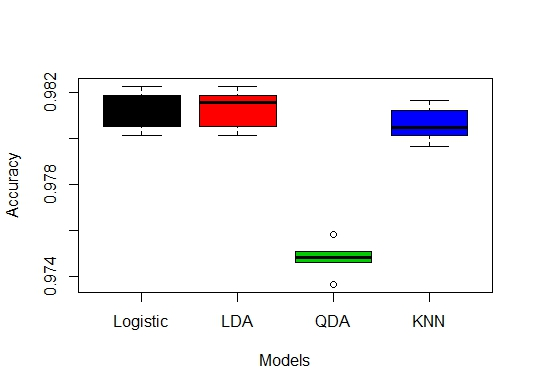
\includegraphics[width=0.45\textwidth]{images/5Fold.jpeg}
	\caption{Accuracies for 5-Fold CV}
	\label{fig:5f}
\end{figure}


\end{document}
